\documentclass[serif]{beamer} %
%\usepackage{pxfonts} % Or palatino or mathpazo packages
%\usepackage{eulervm}


%\documentclass{beamer}
\begin{document}
\title{Overhanging block stacks}   
\subtitle{}
\author{Dr Killian O'Brien}
\date{September 2025} 

\frame{\titlepage} 

\section{Building Challenge}
\frame{
\frametitle{The challenge}
Make a tower of bricks ...  \\
\hfill ... with as much of an overhang as you can.
}

\frame{
\frametitle{An optimal solution for simple stacking}
\begin{block}{A couple of basic principles}
\begin{itemize}
\item
A body balances on a flat surface if its centre of gravity lies over the `footprint'.
\item
Determine the (horizontal) location of a stack's centre of gravity by `averaging' over the locations of centres of the blocks.
\end{itemize}
\end{block}
\begin{block}{Iterate the following construction}
\begin{itemize}
\item
Build by adding to the bottom of the pile
\item
When adding a block, position its edge directly under the centre of gravity of the existing stack.
\end{itemize}
\end{block}
}

\section{Analyzing the solution} 
\frame{
\frametitle{Analyzing the solution}
\begin{block}{Defining $h_n$}
Let $h_n$ denote the overhang of this optimal simple stack of $n$ blocks, each of width $w$.
\begin{center}
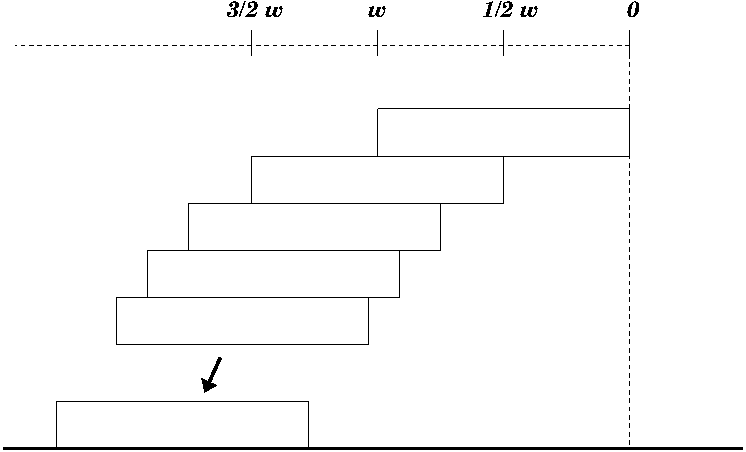
\includegraphics[height=4cm]{stack.png}
\end{center}
\begin{align*}
h_n &= \text{ centre of gravity of the upper $n-1$ blocks}
\end{align*}
\end{block}
}

\frame{
\frametitle{Analyzing the solution}
\begin{block}{A recurrence formula for $h_n$}
\begin{center}
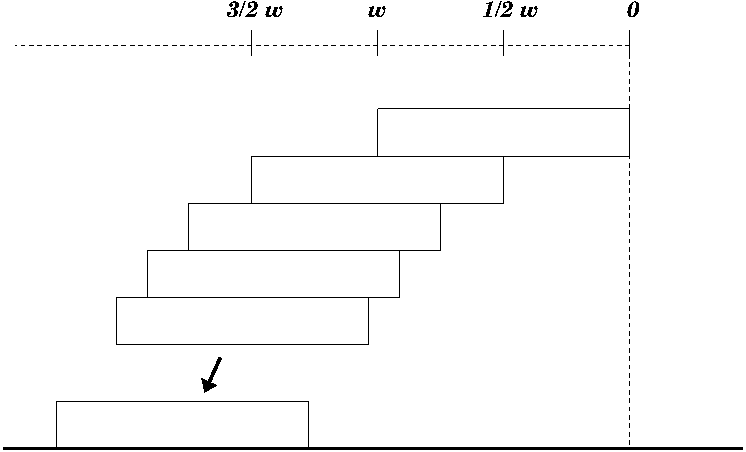
\includegraphics[height=4cm]{stack.png}
\end{center}
\begin{align*}
h_1 & = 0 , \\
h_n &= h_{n-1} + \frac{1}{n-1} \frac{w}{2}
\end{align*}
\end{block}
}

\frame{
\frametitle{Analyzing the solution}
$$h_n = h_{n-1} + \frac{1}{n-1} \frac{w}{2}$$
\begin{block}{Developing $h_1$, $h_2$, \dots}
\begin{align*}
h_1 & = 0 , \\
h_2 &= \frac{w}{2}, \\
h_3 &= \frac{w}{2} + \frac{1}{2} \frac{w}{2} = \frac{w}{2} \left ( 1 + \frac{1}{2} \right ) , \\
h_4 &= \frac{w}{2} \left ( 1 + \frac{1}{2} \right ) + \frac{1}{3} \frac{w}{2} = \frac{w}{2} \left ( 1 + \frac{1}{2} + \frac{1}{3} \right ) \\
&\vdots \\
h_n &= \frac{w}{2} \left (  1 + \frac{1}{2} + \frac{1}{3} + \dots + \frac{1}{n-1} \right )
\end{align*}
\end{block}
}

\frame{
\frametitle{A nice formula for $h_n$ involving the harmonic series}
\begin{block}{But how does it behave as $n$ increases?}
$$h_n = \frac{w}{2} \left (  1 + \frac{1}{2} + \frac{1}{3} + \dots + \frac{1}{n-1} \right )$$
In fact, $1 + \frac{1}{2} + \frac{1}{3} + \dots + \frac{1}{n-1}$ increases without any upper bound. Proof of this based on grouping the terms together in groups of size $2,4,8,16,\dots$
\begin{align*}
& 1 + \frac{1}{2} + \left ( \frac{1}{3} + \frac{1}{4} \right ) + \left ( \frac{1}{5} + \dots + \frac{1}{8} \right )  + 
\left ( \frac{1}{9} + \dots + \frac{1}{16} \right ) + \dots \\
> & 1 + \frac{1}{2} + \frac{2}{4} + \frac{4}{8} +  \frac{8}{16} + \dots \\
=& 1 + \frac{1}{2} + \frac{1}{2} + \frac{1}{2} + \frac{1}{2} + \dots
\end{align*}
Conclusion: Given enough blocks one can achieve any overhang whatsoever!
\end{block}
}

\frame{
\frametitle{Evaluating $h_n$}
$$h_n = \frac{w}{2} \left (  1 + \frac{1}{2} + \frac{1}{3} + \dots + \frac{1}{n-1} \right )$$
\begin{center}
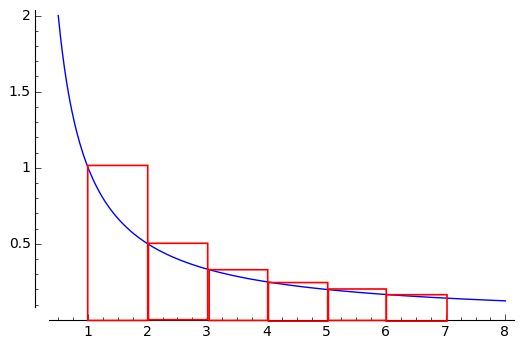
\includegraphics[height=4cm]{integralunfilled.png}
\end{center}
$$h_n \approx \frac{w}{2} \int_1^n \, \frac{1}{x} \, dx $$
}

\frame{
\frametitle{Evaluating $h_n$}
$$h_n \approx \frac{w}{2} \int_1^n \, \frac{1}{x} \, dx $$
\begin{center}
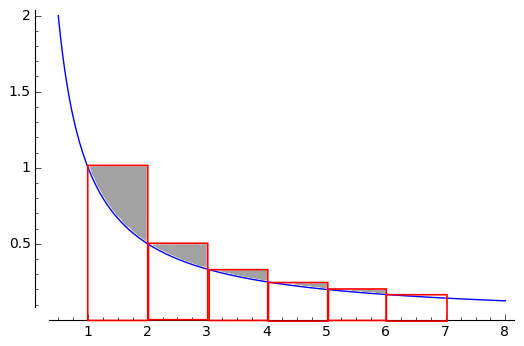
\includegraphics[height=4cm]{integralfilled.png}
\end{center}
$$h_n = \int_1^n \, \frac{1}{x} \, dx + \gamma_n,$$
where 
$$\gamma_n = \text{ area of shaded regions }$$
}

\frame{
\frametitle{Evaluating $h_n$}
$$h_n = \frac{w}{2} \left ( \int_1^n \, \frac{1}{x} \, dx + \gamma_n \right ),$$
\begin{center}
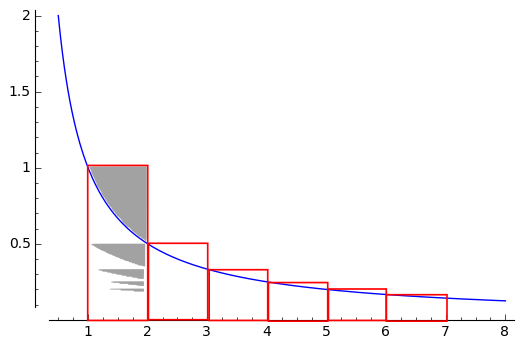
\includegraphics[height=4cm]{integralfilledslid.png}
\end{center}
$$ \lim_{n \to \infty} \gamma_n = \gamma \approx 0.6$$
$\gamma$ is the Euler–Mascheroni constant.
}

\frame{
\frametitle{Evaluating $h_n$}
So for large $n$ a very good approximation is 
\begin{align*}
h_n &\approx \frac{w}{2} \left ( \int_1^n \, \frac{1}{x} \, dx + 0.6 \right ), \\
&= \frac{w}{2} \Big ( \log(n)+ 0.6 \Big ).
\end{align*}
}

\frame{
\frametitle{An actual stack of Jenga blocks}
$$h_n \approx \frac{w}{2} \Big ( \log(n)+ 0.6 \Big )$$
\begin{block}{How tall is a simple optimal stack with a $3$ metre overhang?}
The Jenga block is $7.5$cm wide and $1.5$cm tall.
$$3 = \frac{0.075}{2} \Big ( \log(n) + 0.6 \Big )$$
Solve this to find number, $n$, of blocks required.
\begin{align*}
n &= e^{\left ( \frac{3}{0.0375} - 0.6 \right )} \\
&\approx 3.0 \times 10^{34}, \text{ a LOT of bricks}
\end{align*}
Such a stack would be $3.0 \times 10^{34} \times 0.015 \approx 4.6 \times 10^{32}$ metres tall.
\end{block}
}

\frame{
\frametitle{Now that's tall!}
$4.6 \times 10^{32}$ metres is approximately $520 \, 000$ times the diameter of the observable universe.
}

\end{document}

